\subsubsection{Gain and Frequency Response of Common-Emitter Amplifier}
This portion of the experiment demonstrates the amplification behavior of the inverter, also known as a common-emitter amplifier. Its properties are characterized by analyzing its gain and frequency response. \\
% Initial settings
The amplifier's input signal has a $200$\si{\milli\volt}pp amplitude and an $800$\si{\milli\volt}pp offset.
% At what point do distortions occur?
When the amplitude is increased to $400$\si{\milli\volt}pp, distortions occur in which the waveform becomes clipped. This is because the output waveform is amplified, but its peak and trough voltages are limited by the supply and ground voltages, respectively.
\FloatBarrier
\begin{figure}[h!]
	\centering
	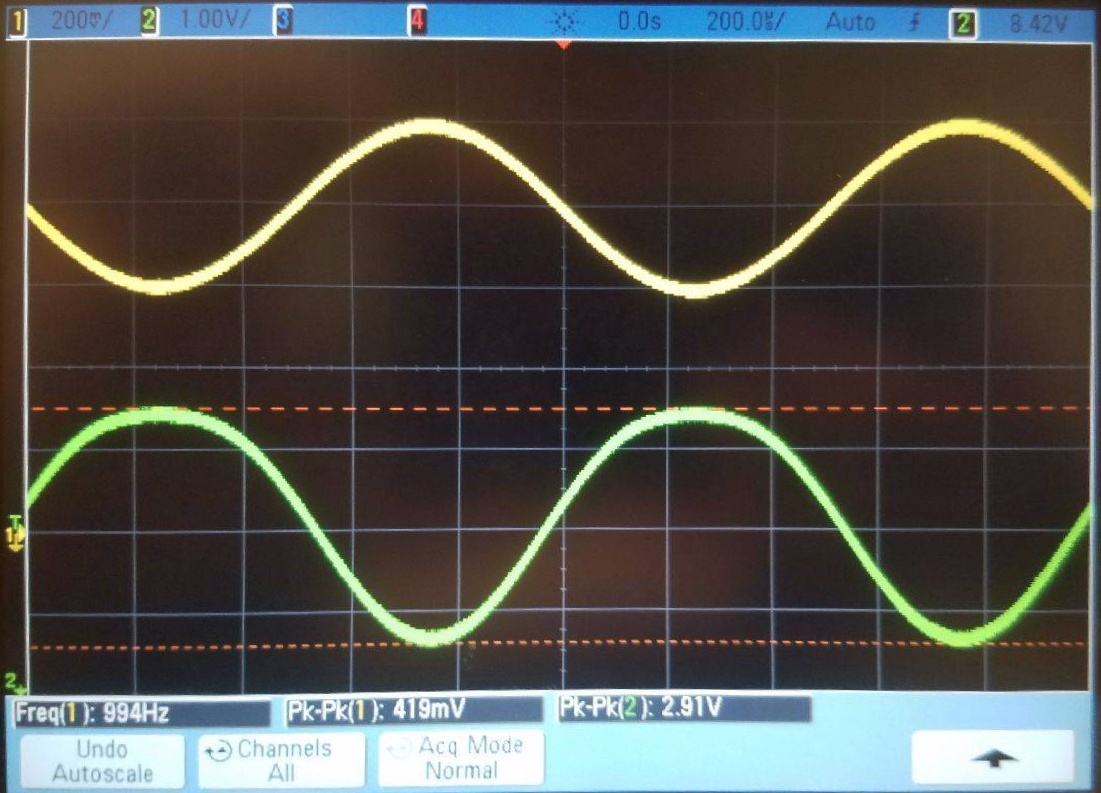
\includegraphics[scale=0.25]{../images/amplifier_10ghz_clamping.jpeg}
	\caption{Common-Emitter Amplifier $10$\si{\kilo\hertz} Distortions}
	\label{fig:clamping}
\end{figure}
\FloatBarrier
% Explanation of low-pass filtering with circuit diagram
The amplifier does not have a perfect frequency response due to the structure of the BJT used. The BJT has two pn-junctions, one between the collector and the base and one between the base and the emitter. Due to a variety of effects, the junctions each have an associated capacitance. At DC, current can easily flow through the BJT. Thus, these capacitances are not accurately modeled using a series capacitance since that would simply charge. A better model uses parallel capacitances, like in figure (\ref{fig:bjt_circ}) below:

\FloatBarrier
% NOTE: Circuit schematics MUST have labeled values.
\begin{figure}[h!]
	\centering
	\caption{High Frequency BJT Model}
	\label{fig:hf_bjt}
	\begin{circuitikz}
		\draw
		( 0 , 0 ) node[ npn ] (my_npn) {}

		% Base
		(my_npn.B) to [ short ] +( -3 , 0 ) coordinate(r_in)
		(r_in) to [ R={$10k\Omega$} ] ++( -3 , 0 ) coordinate(v_in)
		(v_in) to [ battery , v<=$V_{in}$ ] ++( 0 , -2 ) coordinate(gnd_1)
		(gnd_1) node[ ground ] (my_gnd_1) {}

		% Collector
		(my_npn.C) to [ short ] ++( 0 , 3 ) coordinate(r_c)
		(r_c) to [ R={$1k\Omega$} ] ++( 0 , 3 ) coordinate(vcc)
		(vcc) to [ battery , v<=$V_{cc}$ ] ++( 2 , 0 ) coordinate(gnd_3)
		(gnd_3) node[ ground ] (my_gnd_3) {}

		% Emitter
		(my_npn.E) to [ short ] ++( 0 , -3 ) coordinate(e_gnd)
		(e_gnd) node[ ground ] (my_e_gnd) {}

		% Parasitic Capacitances
		(r_c) to [ C ] (r_in)
		(my_e_gnd) to [ C ] (r_in)

		;
	\end{circuitikz}
\end{figure}

\FloatBarrier

At low frequencies, the parasitic capacitances acts as broken circuits. Thus, the circuit reduces to an ideal common-emitter amplifier. However, at higher frequencies, signals can short through the parasitic capacitances. Specifically, a short path exists between ground and the collector, making $V_{out} = 0$\si{\volt}. Thus, as frequency increases, the output voltage for a given input voltage, and therefore the gain, should drop. This is because gain is defined as $\frac{V_{out}}{V_{in}}$ [\ref{ref:bjt_cap}].

% Gain at 10kHz
At $10$\si{\kilo\hertz}, the input voltage is the starting value of $200$\si{\milli\volt}pp, and the output voltage is 1.63\si{\volt}pp. Thus, the gain is $8.15$.
% How do you measure higher cutoff frequency?
Since parasitic capacitances should drop the gain at higher frequencies, a cutoff frequency can be defined. The cutoff frequency $f_c$ is the frequency at which the output voltage is $\frac{1}{\sqrt{2}}$ of the peak output voltage for a given input voltage [\ref{ref:cutoff_freq}]. So, in this case, $f_c$ is the frequency at which the output voltage is $\frac{1.63}{\sqrt{2}}$ \si{\volt}pp $ \approx 1.15$ \si{\volt}pp. This can be measured by simply increasing the frequency until an output voltage amplitude of $1.15$ \si{\volt}pp occurs.
% What was our measured cutoff frequency?
Using this method, the cutoff frequency $f_c \approx 150$\si{\kilo\hertz} is obtained.
% Gain at cutoff frequency
At this point, the gain is approximately $5.75$.
% Table with gains at different frequencies
\FloatBarrier
\begin{table}[h!]
	\centering
	\caption{Common-Emitter Amplifier Frequency Response}
	\label{tab:cea_response}
	\csvautotabular{../tables/amplifier_gains.csv}
\end{table}
\FloatBarrier
\subsubsection{Square Wave Response of Common-Emitter Amplifier}
% Output signal vs square wave input
The frequency of the square wave response is set to the cutoff frequency $f_c = 150$\si{\kilo\hertz}. In order to understand the square wave response of a common-emitter amplifier, the 20\% duty cycle case is considered first.
\FloatBarrier
\begin{figure}[h!]
	\centering
	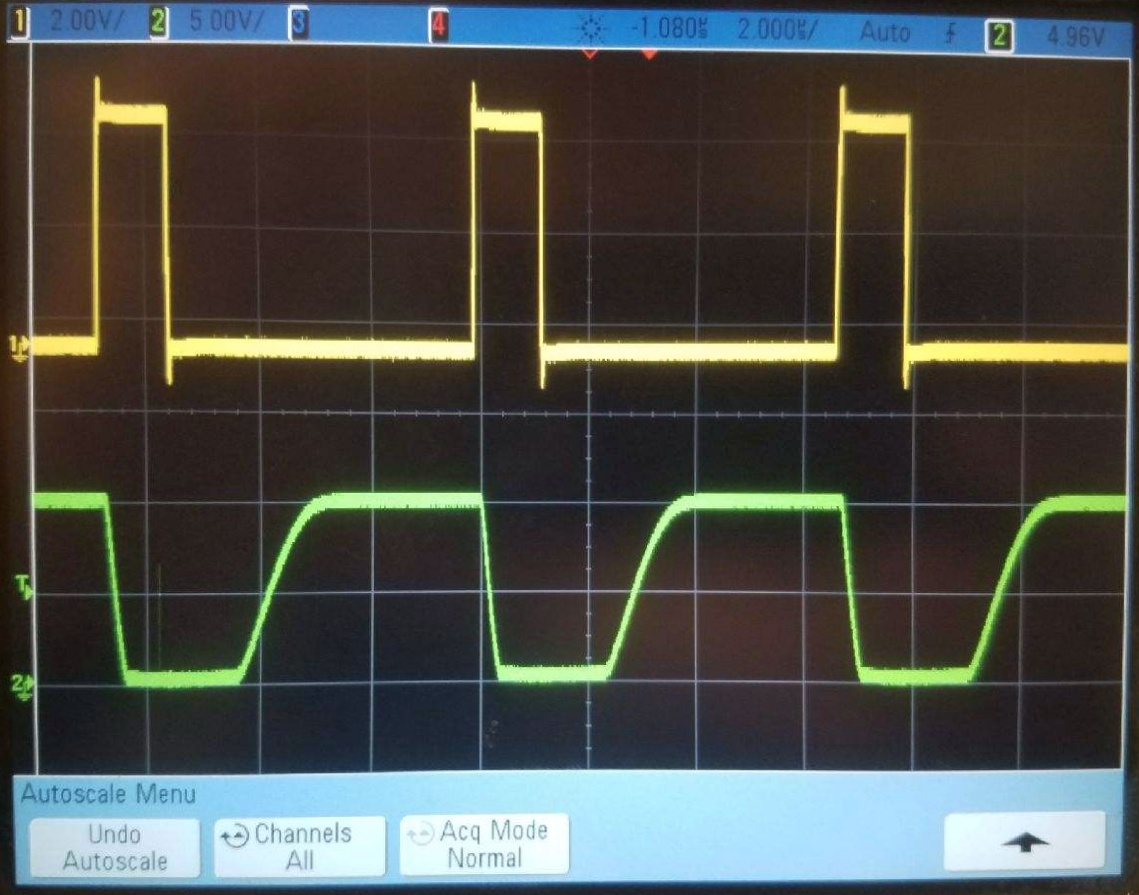
\includegraphics[scale=0.25]{../images/amplifier_20_duty_cycle.jpeg}
	\caption{Common-Emitter Amplifier Square Wave Response 20\% Duty Cycle}
	\label{fig:twenty_perc_duty_cycle}
\end{figure}
\FloatBarrier
When the square wave pulse is high, the output drops nearly to ground due to the inverting characteristics of the amplifier. When the input drops to ground, the output gradually becomes high for the same reason. There is a brief delay between the falling edge of the input waveform and the rising "edge" of the output waveform. This is because the capacitors in figure (\ref{fig:hf_bjt}) need to charge first before the low-pass filter's DC characteristics take over. The charging and discharging of the capacitors represents the formation and destruction of the depletion regions in the BJT. \\
The reason the output waveform appears to saturate is because the duty cycle is low enough that the input signal remains low for long enough that a steady state can be established. It saturates at $10$\si{\volt}, the supply voltage, because the output voltage cannot exceed supply. The amplifier operates on the principle of using the weaker signal to enable or disable a transistor switch that controls a larger voltage. This larger voltage is the supply voltage, which is why the output cannot exceed supply. \\
When the duty cycle is increased to 50\%, the same physical principles still apply.
\FloatBarrier
\begin{figure}[h!]
	\centering
	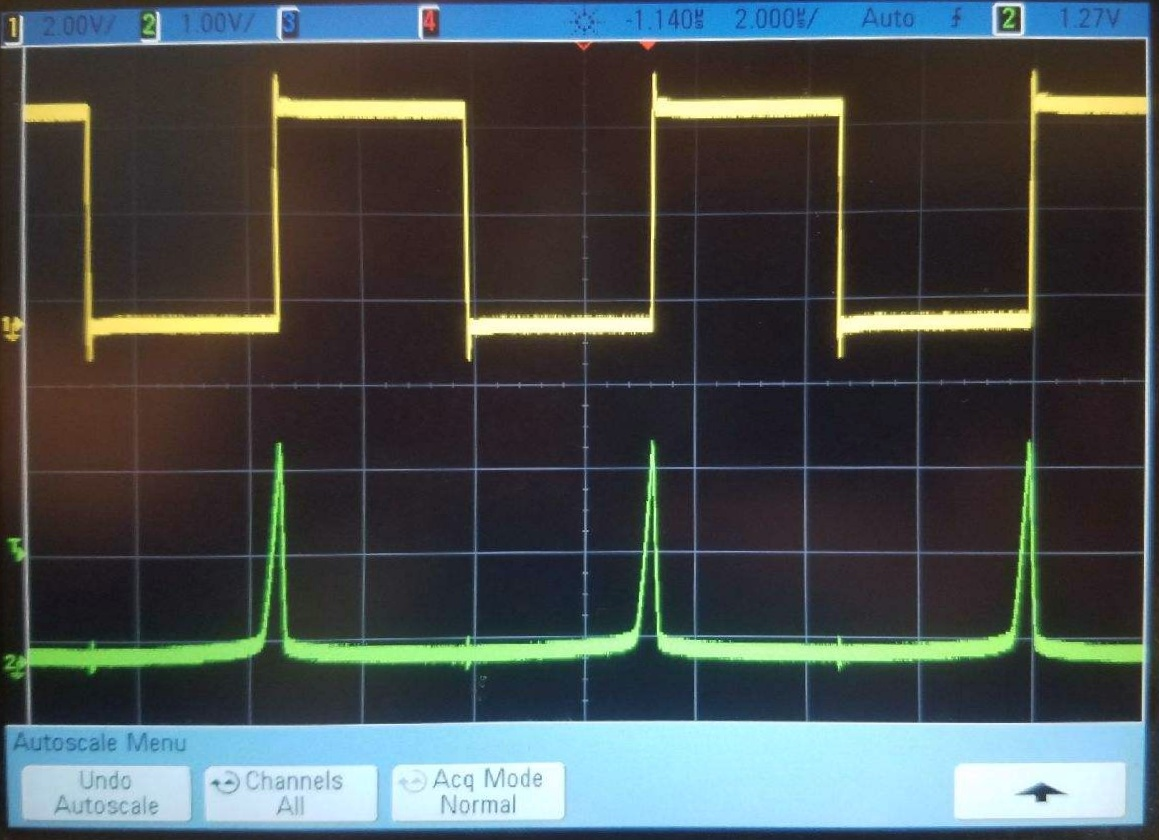
\includegraphics[scale=0.25]{../images/amplifier_50_duty_cycle.jpeg}
	\caption{Common-Emitter Amplifier Square Wave Response 50\% Duty Cycle}
	\label{fig:fifty_perc_duty_cycle}
\end{figure}
\FloatBarrier
The output waveform waits for a time delay and then begins to develop. However, because the duty cycle is longer, the input signal remains low for a shorter period of time. Thus, the output voltage does not have a sufficient amount of time to fully develop and is cut short when the rising edge of the input occurs. \\
% Why is there distortion
% TODO Add values to circuit schematics. TODO Discussion. TODO Tell Jason to put values in circuit schematics and explain why inverting amplifier works. Send him your prelab which explains why.

% References
References \\
\url{http://www.ittc.ku.edu/~jstiles/412/handouts/5.8\%20BJT\%20Internal\%20Capacitances\%20and\%20high\%20frequency\%20model/section\%205_8\%20BJT\%20Internal\%20Capacitances\%20lecture.pdf} \\ %ref:bjt_cap
\url{http://alignment.hep.brandeis.edu/Lab/Filter/Filter.html} \\ %ref:cutoff_freq
